\begin{figure}[H]
	\centering
	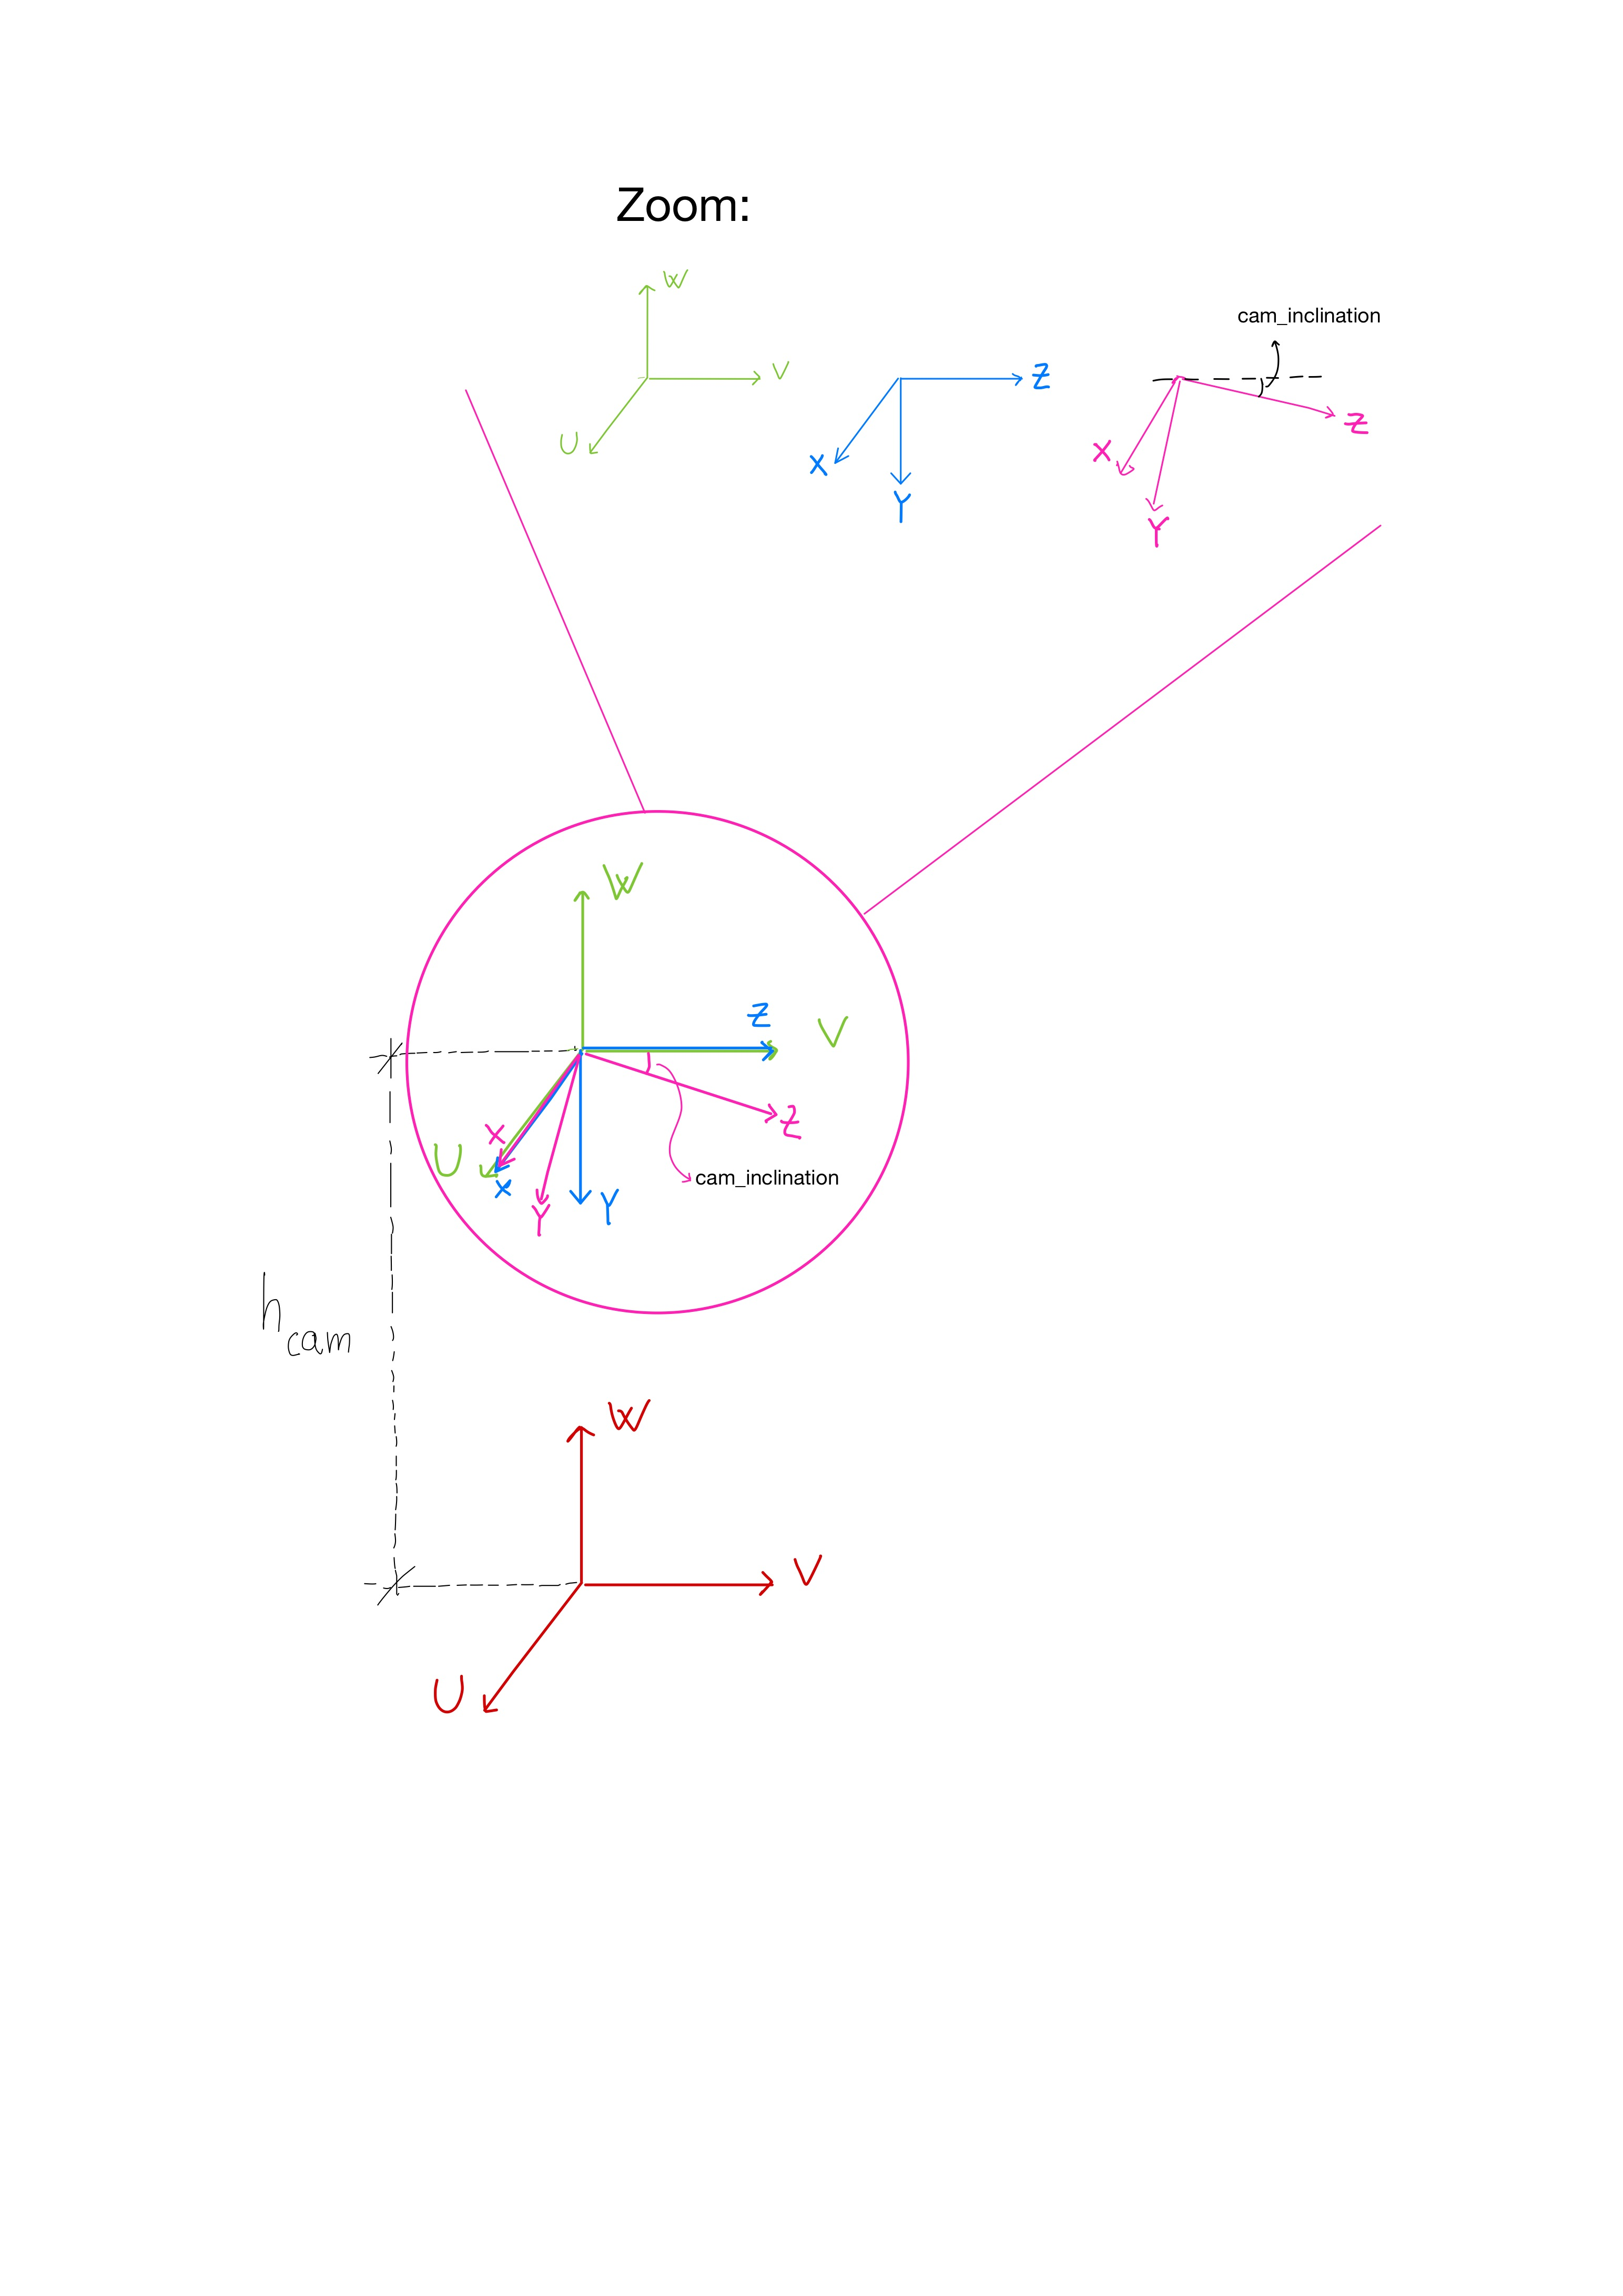
\includegraphics[width=0.8\textwidth]{Immagini/RoboticsFrames-2.jpg}
	\caption{Frames scelti}
	\label{fig:frames}
\end{figure}


Le seguenti sono le matrici utilizzate nel codice per rappresentare le rotazioni dei sistemi di riferimento.
\begin{lstlisting}
R_traslation << 1,0,0,0,
				0,1,0,0,
				0,0,1,-h_cam,
				0,0,0,1;

R_rot_cam_inclination  << 1,0,0,0,
					      0,cos(cam_inclination),-sin(cam_inclination),0,
						  0,sin(cam_inclination),cos(cam_inclination),0,
						  0,0,0,1;

R_rot_camera << 1,0,0,0,
				0,cos(M_PI/2),-sin(M_PI/2),0,
				0,sin(M_PI/2),cos(M_PI/2),0,
				0,0,0,1;
\end{lstlisting}